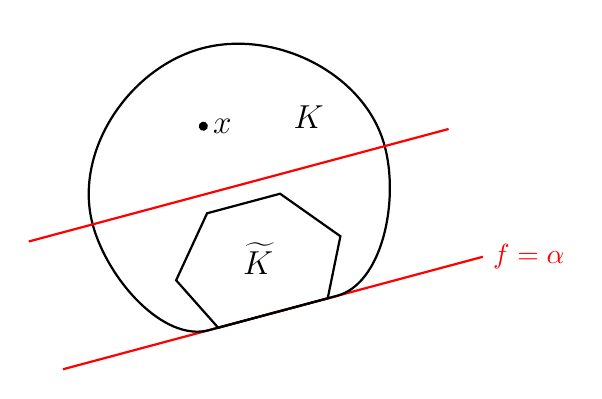
\begin{tikzpicture}[scale=1.2, rotate=15] % 整体旋转15度，还原手绘的倾斜感

    % 1. 绘制底部的支撑超平面 f = \alpha (红色平行线)
    % 设底线在 y = -1 的水平线上。红线比公用底边长。
    \draw[thick, red] (-2.3, -1) -- (2.3, -1) node[right, text=red] {$f=\alpha$};

    % 2. 绘制外部的大凸集 K (极致平滑的新形状)
    % 中心大约在 (0, 0.45)，外围半径约 1.6-1.7
    % 使用全贝塞尔路径实现圆弧和直线的自然平滑过渡，确保在底部与 y = -1 完全公用共线。
    % 通过更柔和的控制点实现极致自然平滑的过渡。
    \draw[thick] (-0.7, -1) -- (0.7, -1) % 公用底边
          .. controls (1.2, -1) and (1.6, -0.2) .. (1.6, 0.4) % 右下平滑过渡，圆弧切点在 (1.6, 0.4)
          .. controls (1.6, 1.2) and (0.8, 1.9) .. (0, 1.9) % 顶部圆弧
          .. controls (-0.8, 1.9) and (-1.6, 1.2) .. (-1.6, 0.4) % 左上圆弧，圆弧切点在 (-1.6, 0.4)
          .. controls (-1.6, -0.2) and (-1.2,-1) .. cycle; % 左下平滑过渡，回到底边
    % 标签在大凸集 K 的主体上
    \node[font=\large] at (0.9, 0.9) {$K$};

    % 3. 绘制内部的小凸集 (对应证明中的 \tilde{K})
    % 凸多边形，底边 (-0.6, -1) -- (0.6, -1) 严格落在 y = -1 的公用边上。
    \draw[thick] (-0.6, -1) -- (0.6, -1) -- (0.9, -0.4) -- (0.4, 0.2) -- (-0.4, 0.2) -- (-0.9, -0.4) -- cycle;
    % 标签在内部小图形上
    \node[font=\large] at (0, -0.4) {$\widetilde{K}$};

    % 4. 绘制中间的分离超平面 (红色平行线)
    % 同一个泛函 f 的等值线，必然与 y = -1 严格平行，通过 y = 0.4
    \draw[thick, red] (-2.3, 0.4) -- (2.3, 0.4);

    % 5. 绘制极点 x (对应证明中的点 c)
    % 确保它位于分离超平面上方，大凸集内部
    \filldraw (-0.2, 1.1) circle (1.2pt);
    \node[right, font=\large] at (-0.2, 1.1) {$x$};

\end{tikzpicture}